\documentclass[12pt,a4paper]{article}

\usepackage{Act}
\usepackage{listings}

\begin{document}
\input{\detokenize{/home/fenarius/Travail/Cours/Commun/latex/Macros.tex}}

\EP{7}{2022--2023}
\pythonmode

\Exo{Minimum des éléments d'une liste}{}

Ecrire une fonction {\tt minimum} qui prend en argument une liste d'entiers \textit{non vide} {\tt entiers} et renvoie le minimum des éléments de cette liste. 


\textbf{Exemples :}
\begin{lstlisting}
>>> minimum([12,11,8,20,15])
8
>>> minimum([5,-12,0,1,-4,7])
-12
>>> minimums([7,11,2])
2
>>> minimums([3])
3
\end{lstlisting}

\vspace{0.2cm}

\Exo{Codage de César}{}

Etant donné un nombre entier {\tt cle} compris entre 1 et 25, le chiffrement de César ou chiffrement par décalage consiste à décaler chaque lettre de {\tt cle} emplacement dans l'alphabet. Par exemple dans l'illustration suivante {\tt cle} vaut 3. 
\begin{center}
    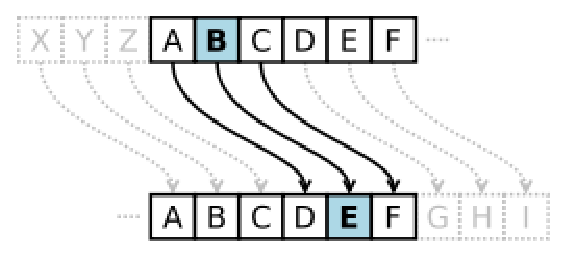
\includegraphics[width=250px]{cesar.eps}
\end{center}
Avec un décalage de 3 on a donc : A qui devient D, B qui devient E, \dots, X qui devient A, Y qui devient B, Z qui devient C.
On veut écrire une fonction {\tt chiffre} qui prend en argument une clé  {\tt cle} et un texte {\tt texte}  et renvoie ce texte chiffré avec le chiffrement de César. On suppose que le texte est \textit{uniquement} constitué de lettres majuscules non accentuées. On propose l'algorithme suivant pour coder un caractere :
\begin{itemize}
    \item Utiliser la fonction {\tt ord} de Python pour obtenir son code
    \item Augmenter le code de {\tt cle} et soustraire 26 si on dépasse le code de la lettre Z.
    \item Utiliser la fonction {\tt chr} de Python pour obtenir la lettre codée.
\end{itemize} 

\begin{lstlisting}
    def chiffre(texte,cle):
    ''' Renvoie le chiffrement de texte par decalage de cle emplacements'''
    texte_code = ....
    for caractere in .....:
        num = .......
        num = num + .....
        if ..... > ......:
            num=........
        texte_code = texte_code + .......
    return ......
\end{lstlisting}

\textbf{Exemples}
\begin{lstlisting}
>>> chiffre("NSI",3)
QVL
>>> chiffre("MATHS",12)
YMFTE
\end{lstlisting}
\end{document}
